\documentclass[a4paper, 12pt]{article}

% Добавляем новые пакеты
\usepackage[english, russian]{babel}    % Пакет для поддержки русского языка
\usepackage[T1, T2A]{fontenc}           % Загружаем пакет с поддержкой кирилицы
\usepackage[utf8]{inputenc}             % Загружаем пакет с поддержкой кодировки файла и символов
\usepackage{graphicx}                   % Загружаем пакет для добавления различной графики (pdf, jpg, png)
\usepackage{import}                     % Загружаем пакет для продвинутого импорта, в частности изображений pdf_tex из графического редактора inkscape (\import{<path to file>}{<filename>.pdf_tex})
\usepackage{subcaption}                 % Пакет для поддержки сетки из фигур, например в две колонки или матрицей
\usepackage{float}                      % Пакет для улучшенного размещения изображенией (ниже используется опция H в команде \begin{figure}[H])
\usepackage{geometry}                   % Пакет для управления отступами на странице (см. далее вызываем \geometry)
\usepackage{amsmath}                    % Добавляем крутую поддержку математики, в частности /align
\usepackage{amsfonts}                   % Пкет с мтематическими шрифтами вроде \mathbb и др.
\usepackage{tabu}                       % Пакет с прокаченными таблицами
\usepackage{booktabs}                   % Крутые вертикальные разделители
\usepackage[dvipsnames]{xcolor}         % Рассширенная поддержка цветов
\usepackage[colorlinks]{hyperref}
\usepackage{indentfirst}                % Пакет, чтобы починить красную строку
\usepackage{listings}                   % Поддержка листингов, оформления кода программы
\usepackage{src/title}               % Титульный лист (смотри файл vpdtitle.sty)


% Устанавливает отступы на странице
\geometry{left=2cm, right=2cm, bottom=2cm, top=2cm}

% Настараиваем красивые цвета для ссылок на формулы, фигуры (изображения) и другие элементы.
\hypersetup{
    linkcolor=blue,
    filecolor=magenta,
    urlcolor=cyan
}

% Настраиваем супер красивые листинги с попомщью пакетов listings и xcolor
\definecolor{codegreen}{rgb}{0,0.6,0}
\definecolor{codegray}{rgb}{0.5,0.5,0.5}
\definecolor{codepurple}{rgb}{0.58,0,0.82}
\definecolor{backcolour}{rgb}{0.95,0.95,0.92}

\lstdefinestyle{codestyle}{
    backgroundcolor=\color{backcolour},
    commentstyle=\color{codegreen},
    keywordstyle=\color{magenta},
    numberstyle=\tiny\color{codegray},
    stringstyle=\color{codepurple},
    basicstyle=\ttfamily\footnotesize,
    breakatwhitespace=false,
    breaklines=true,
    captionpos=b,
    keepspaces=true,
    numbers=left,
    numbersep=5pt,
    showspaces=false,
    showstringspaces=false,
    showtabs=false,
    tabsize=2
}

\lstset{style=codestyle}
\lstset{extendedchars=\true}


%%%%%%%%%%%%%%%%%%%%%%%%%%%%%%%%%%%%%%%%%%%%%%%%
%% Заполнение титульного листа (оригинал)
%%%%%%%%%%%%%%%%%%%%%%%%%%%%%%%%%%%%%%%%%%%%%%%%
\title{
    Лабораторная №2\\
    Определение параметров двигателя EV3 на основе вольтамперной характеристики
}

\author{Ануфриев А. С.\\Ндава Маргарет Чити\\Глаголев М.К.}
\affil{
    465029, \href{https://t.me/me_and_no_oneelse}{@me\_and\_no\_oneelse}\\
    505413, \href{https://t.me/margaritaanybody}{@margaritaanybody}\\
    504722, \href{https://t.me/R07331821}{@R07331821}}
\supervisor{\href{https://my.itmo.ru/persons/192059}{Овчаров Алексей Олегович}
}
\abstract{
    В данной работе экспериментально определены\\
    параметры модели электродвигателя постоянного тока Lego EV3. Сняты\\
    переходные процессы угла и скорости при 18 уровнях управляющего сигнала\\
    в диапазоне от $-50\%$ до $+50\%$. Определены статический коэффициент\\
    передачи $k$ и постоянная времени $T_m$ методом наименьших квадратов.\\
    Построена вольтамперная характеристика. Оценены параметры $R$, $J$,\\
    $k_e$, $k_m$. Результаты сравнены с данными лабораторной работы №1.
}
\keywords{
    ДПТ; Идентификация; Вольтамперная характеристика; Python; MATLAB
}

\date{05.04.2026}

%%%%%%%%%%%%%%%%%%%%%%%%%%%%%%%%%%%%%%%%%%%%%%%%
% Начало документа
%%%%%%%%%%%%%%%%%%%%%%%%%%%%%%%%%%%%%%%%%%%%%%%%
\begin{document}

    \newpage
    \maketitle
    \newpage
    \tableofcontents
    \newpage


\section{Постановка задачи}

\subsection{Цель и задачи исследования}

Цель работы — экспериментальное определение параметров электродвигателя постоянного тока Lego EV3 на основе полной математической модели, учитывающей электромагнитные процессы.

Задачи:
\begin{enumerate}
    \item Изучить полную математическую модель двигателя постоянного тока с учётом индуктивности обмоток.
    \item Снять вольтамперную характеристику (зависимость напряжения от тока) при заторможенном роторе для 18 уровней управляющего сигнала.
    \item Определить активное сопротивление обмоток $R$ методом наименьших квадратов.
    \item Снять переходные процессы угла поворота $\theta(t)$ и угловой скорости $\omega(t)$ при ступенчатом воздействии.
    \item Определить момент инерции ротора $J$ на основе геометрических параметров и передаточного отношения редуктора.
    \item Вычислить конструктивные постоянные двигателя $k_e$ и $k_m$.
    \item Построить Simulink-модель и верифицировать полученные параметры.
\end{enumerate}

\subsection{Объект исследования}

Объектом исследования является мотор-редуктор Lego Mindstorms EV3 (Large Motor), который представляет собой устройство, содержащее электродвигатель постоянного тока с постоянными магнитами, редуктор с передаточным отношением $i = 48$, датчик угла поворота и управляющую микросхему.

\begin{figure}[H]
    \centering
    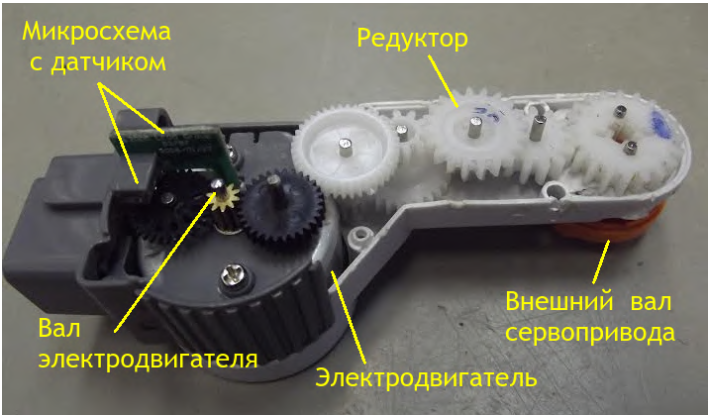
\includegraphics[width=0.7\textwidth]{picture_8.png}
    \caption{Мотор-редуктор EV3 в разобранном виде.}
    \label{fig:motor_disassembled}
\end{figure}

\section{Теоретическая часть}

\subsection{Полная математическая модель двигателя}

В технических задачах, связанных с автоматическим управлением, все явления рассматриваются как процессы, характеризующиеся входными сигналами (управляющие воздействия) и выходными сигналами (наблюдаемые величины). Для электродвигателя входным сигналом является подаваемое напряжение $U_{\text{ctrl}}$, а выходными — угловая скорость $\omega(t)$ и сила тока $I(t)$.

При составлении полной математической модели необходимо учитывать не только ЭДС индукции со стороны поля статора, но и ЭДС самоиндукции, возникающую из-за изменения магнитного потока в катушках ротора.

\subsection{Физические законы}

\paragraph{Второй закон Ньютона для вращательного движения:}
\begin{equation}
    J \frac{d\omega(t)}{dt} = M_{\text{em}}(t) - M_{\text{нагр}}(t),
\end{equation}
где $J$ — момент инерции ротора (кг·м$^2$), $\omega$ — угловая скорость (рад/с). В режиме холостого хода $M_{\text{нагр}} = 0$.

Электромагнитный момент:
\begin{equation}
    M_{\text{em}}(t) = k_m I(t),
\end{equation}
где $k_m$ — коэффициент момента (Н·м/А).

\paragraph{Закон Ома с учётом ЭДС:}
При вращении ротора в обмотке возникает ЭДС индукции со стороны поля статора $\mathcal{E}_{\text{stat}} = -k_e\omega$, а также ЭДС самоиндукции $\mathcal{E}_{\text{self}} = -L\dot{I}$. Полный закон Ома принимает вид:
\begin{equation}
    U_{\text{ctrl}} + \mathcal{E}_{\text{stat}} + \mathcal{E}_{\text{self}} = I R,
\end{equation}
или
\begin{equation}
    U_{\text{ctrl}} - k_e\omega - L\frac{dI}{dt} = I R.
\end{equation}

\subsection{Система дифференциальных уравнений}

Объединяя уравнения, получаем систему в форме «вход-состояние»:
\begin{equation}
    \begin{cases}
        \dot{\omega} = \dfrac{k_m}{J} I, \\[10pt]
        \dot{I} = \dfrac{1}{L} U_{\text{ctrl}} - \dfrac{k_e}{L} \omega - \dfrac{R}{L} I.
    \end{cases}
\end{equation}

В матричной форме:
\begin{equation}
    \begin{bmatrix} \dot{\omega} \\ \dot{I} \end{bmatrix} =
    \begin{bmatrix} 0 & \dfrac{k_m}{J} \\ -\dfrac{k_e}{L} & -\dfrac{R}{L} \end{bmatrix}
    \begin{bmatrix} \omega \\ I \end{bmatrix} +
    \begin{bmatrix} 0 \\ \dfrac{1}{L} \end{bmatrix} U_{\text{ctrl}}.
\end{equation}

\subsection{Модель «вход-выход»}

Исключая ток, можно получить дифференциальное уравнение второго порядка:
\begin{equation}
    \frac{L}{R} \ddot{\omega} + \dot{\omega} + \frac{k_m k_e}{JR} \omega = \frac{k_m}{JR} U_{\text{ctrl}}.
\end{equation}

Вводятся две постоянные времени:
\begin{itemize}
    \item Электромагнитная постоянная времени: $T_s = \dfrac{L}{R}$,
    \item Электромеханическая постоянная времени: $T_m = \dfrac{JR}{k_m k_e}$.
\end{itemize}

Тогда уравнение принимает вид:
\begin{equation}
    T_s T_m \ddot{\omega} + T_m \dot{\omega} + \omega = \frac{1}{k_e} U_{\text{ctrl}}.
\end{equation}

При $L = 0$ ($T_s = 0$) модель упрощается до апериодического звена первого порядка, рассмотренного в лабораторной работе №1:
\begin{equation}
    T_m \dot{\omega} + \omega = \frac{1}{k_e} U_{\text{ctrl}}.
\end{equation}

\begin{figure}[H]
    \centering
    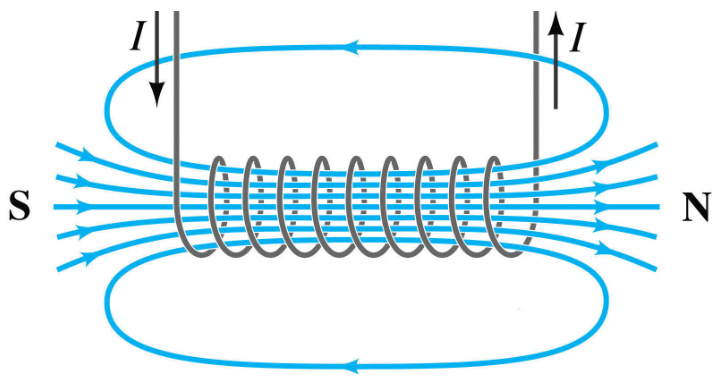
\includegraphics[width=0.8\textwidth]{picture_1.png}
    \caption{Появление индукционных магнитных полей при подаче напряжения.}
    \label{fig:induction}
\end{figure}

\subsection{Особенности мотор-редуктора}

Мотор EV3 содержит редуктор, который изменяет момент инерции, приведённый к выходному валу. На рис.~\ref{fig:gear_model} показана модель редуктора с тремя шестернями.

\begin{figure}[H]
    \centering
    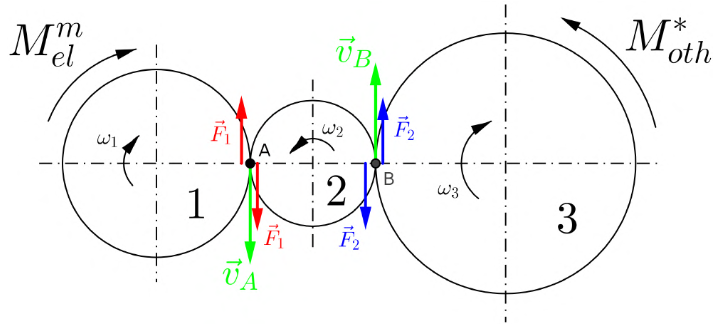
\includegraphics[width=0.6\textwidth]{picture_9.png}
    \caption{Модель мотор-редуктора с тремя шестернями.}
    \label{fig:gear_model}
\end{figure}

Приведённый момент инерции вычисляется по формуле:
\begin{equation}
    J_{\text{real}} = J_1\left(\frac{r_3}{r_1}\right)^2 + J_2\left(\frac{r_3}{r_2}\right)^2 + J_3.
\end{equation}

Пренебрегая моментами инерции шестерён редуктора ($J_2$, $J_3$) по сравнению с моментом инерции якоря двигателя ($J_1$), получаем:
\begin{equation}
    J = J_{\text{якоря}} \cdot i^2,
\end{equation}
где $i = \dfrac{\omega_1}{\omega_3} = 48$ — передаточное отношение редуктора EV3.

\subsection{Вольтамперная характеристика}

При заторможенном роторе ($\omega = 0$) ЭДС индукции отсутствует, и уравнение упрощается:
\begin{equation}
    U_{\text{ctrl}} = I R.
\end{equation}
Это позволяет определить активное сопротивление обмоток $R$ из вольтамперной характеристики.

\section{Экспериментальная установка}

\subsection{Оборудование}

Для проведения эксперимента использовались:
\begin{itemize}
    \item Контроллер Lego Mindstorms EV3;
    \item Мотор-редуктор EV3 (Large Motor);
    \item Специальный кабель с доступом к проводам питания (рис.~\ref{fig:cable});
    \item Цифровой мультиметр для измерения тока и напряжения;
    \item Персональный компьютер с Python и MATLAB/Simulink.
\end{itemize}

\begin{figure}[H]
    \centering
    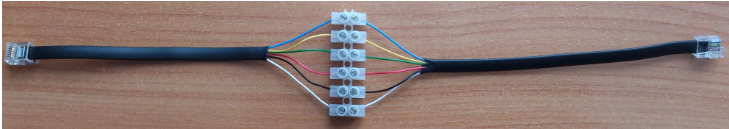
\includegraphics[width=0.5\textwidth]{picture_10.png}
    \caption{Специальный кабель для доступа к проводам питания.}
    \label{fig:cable}
\end{figure}

\begin{figure}[H]
    \centering
    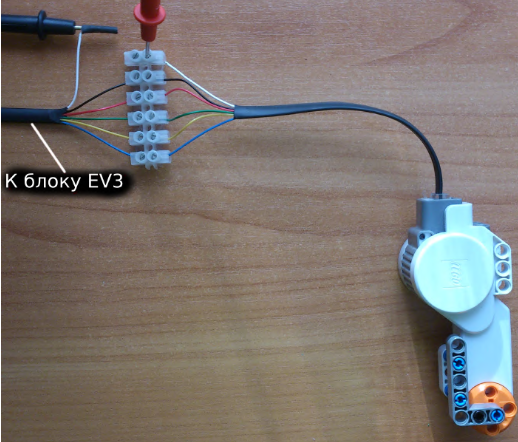
\includegraphics[width=0.7\textwidth]{picture_12.png}
    \caption{Измерение силы тока в цепи двигателя.}
    \label{fig:current_meas}
\end{figure}

\subsection{Методика измерений}

\paragraph{Снятие вольтамперной характеристики:}
Для каждого уровня управляющего сигнала $U \in \{\pm10\%, \pm15\%, \dots, \pm50\%\}$ при заторможенном роторе измерялись напряжение и ток. Измерения проводились для обоих направлений вращения.

\paragraph{Снятие переходных процессов:}
Двигателю подавалось ступенчатое воздействие на 1 секунду. Одновременно записывались время $t$ (с), угол поворота $\theta(t)$ (град) и угловая скорость $\omega(t)$ (град/с). Результаты сохранялись в TXT-файлы для последующей обработки.

\section{Результаты измерений}

\subsection{Вольтамперная характеристика}

Результаты измерений напряжения и тока для 18 уровней управляющего сигнала приведены в табл.~\ref{tab:ui}.

\begin{table}[H]
    \centering
    \caption{Зависимость напряжения от тока при заторможенном роторе}
    \label{tab:ui}
    \begin{tabular}{|c|c|c|}
        \hline
        \textbf{ШИМ, \%} & \textbf{Напряжение $U$, В} & \textbf{Ток $I$, А} \\
        \hline
        $+50$  &  2,75 &  0,63 \\
        $+45$  &  2,53 &  0,56 \\
        $+40$  &  1,99 &  0,51 \\
        $+35$  &  1,92 &  0,45 \\
        $+30$  &  1,68 &  0,37 \\
        $+25$  &  1,36 &  0,31 \\
        $+20$  &  1,19 &  0,26 \\
        $+15$  &  0,95 &  0,20 \\
        $+10$  &  0,61 &  0,12 \\
        \hline
        $-10$  & -0,60 & -0,11 \\
        $-15$  & -0,94 & -0,19 \\
        $-20$  & -1,19 & -0,26 \\
        $-25$  & -1,39 & -0,31 \\
        $-30$  & -1,68 & -0,37 \\
        $-35$  & -1,98 & -0,44 \\
        $-40$  & -2,27 & -0,51 \\
        $-45$  & -2,53 & -0,57 \\
        $-50$  & -2,75 & -0,62 \\
        \hline
    \end{tabular}
\end{table}

На рис.~\ref{fig:ui} представлена вольтамперная характеристика двигателя. Экспериментальные точки хорошо ложатся на прямую линию, что подтверждает омический характер сопротивления обмоток.

\begin{figure}[H]
    \centering
    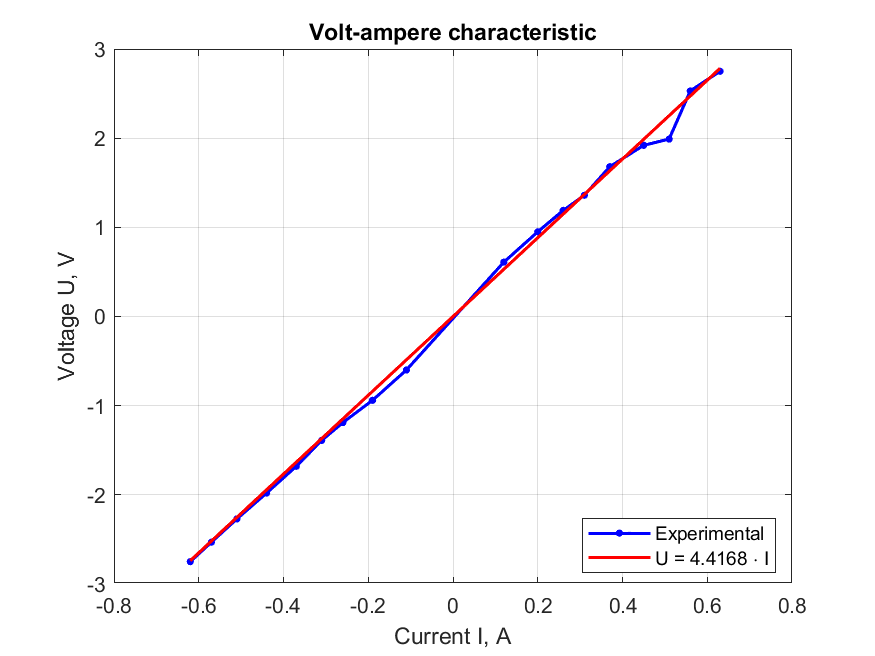
\includegraphics[width=0.9\textwidth]{../matlab/graphs/U_I_dependence.png}
    \caption{Вольтамперная характеристика двигателя: зависимость напряжения от тока.}
    \label{fig:ui}
\end{figure}

\subsection{Переходные процессы}

На рис.~\ref{fig:vel_all} представлены переходные процессы угловой скорости для всех 18 уровней управляющего сигнала. Видно, что скорость нарастает по экспоненциальному закону, что соответствует модели апериодического звена первого порядка.

\begin{figure}[H]
    \centering
    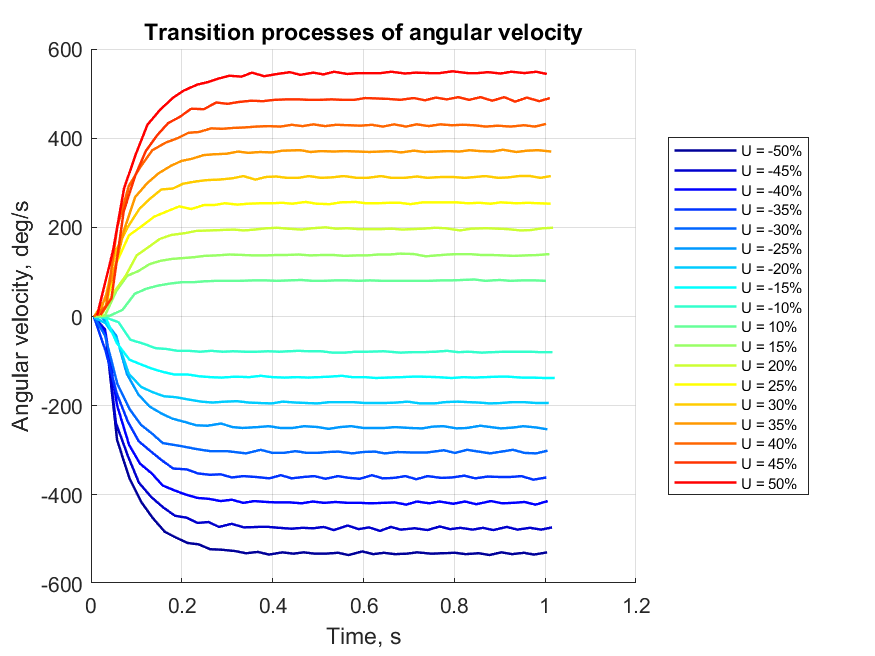
\includegraphics[width=0.95\textwidth]{../matlab/graphs/all_velocities.png}
    \caption{Переходные процессы угловой скорости для всех уровней управляющего сигнала (эксперимент — синий, аппроксимация — красный).}
    \label{fig:vel_all}
\end{figure}

На рис.~\ref{fig:angle_all} представлены переходные процессы угла поворота. Угол нарастает по параболическому закону с экспоненциальной корректировкой в начальный момент.

\begin{figure}[H]
    \centering
    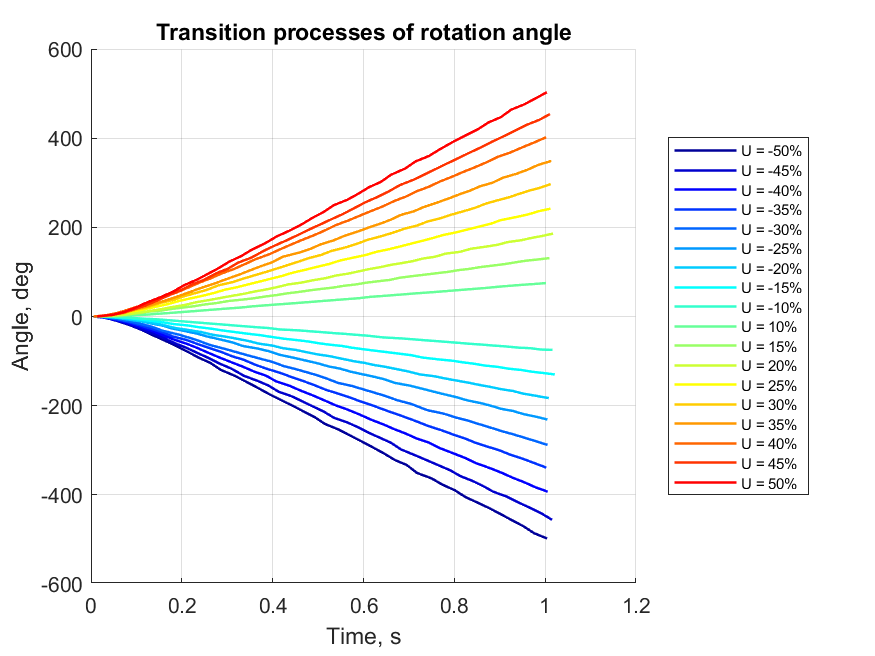
\includegraphics[width=0.95\textwidth]{../matlab/graphs/all_angles.png}
    \caption{Переходные процессы угла поворота для всех уровней управляющего сигнала (эксперимент — синий, аппроксимация — красный).}
    \label{fig:angle_all}
\end{figure}

Пример аппроксимации для одного уровня сигнала показан на рис.~\ref{fig:angle_example}.

\begin{figure}[H]
    \centering
    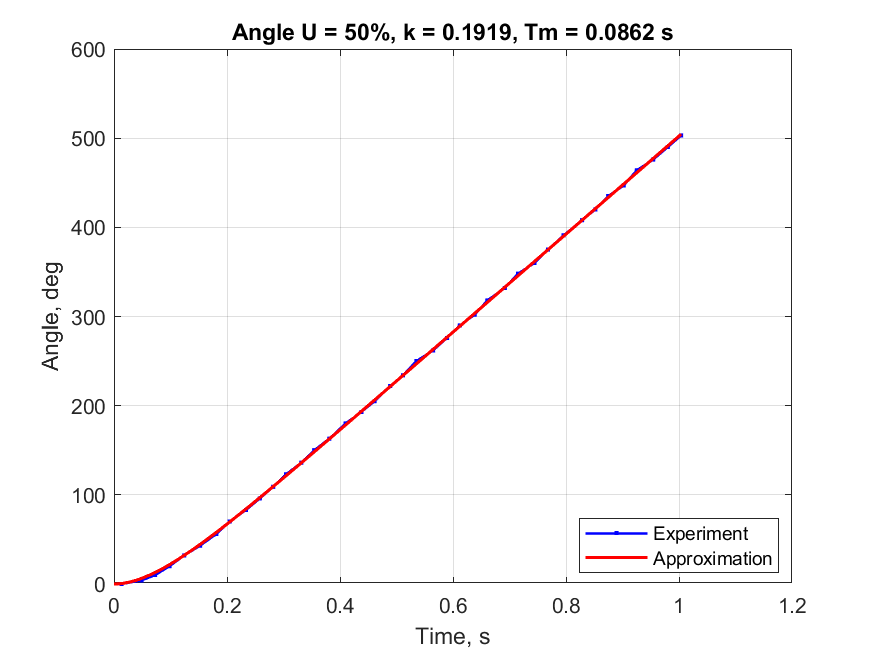
\includegraphics[width=0.8\textwidth]{../matlab/graphs/angles/angle_50.png}
    \caption{Аппроксимация переходного процесса угла поворота при $U = +50\%$.}
    \label{fig:angle_example}
\end{figure}

\begin{figure}[H]
    \centering
    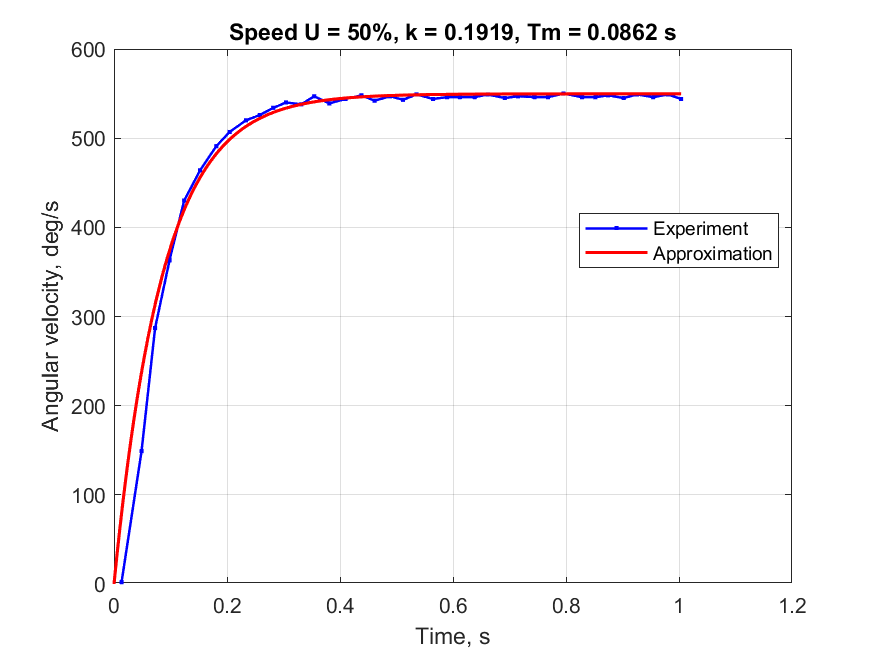
\includegraphics[width=0.8\textwidth]{../matlab/graphs/velocities/velocity_50.png}
    \caption{Аппроксимация переходного процесса угловой скорости поворота при $U = +50\%$.}
    \label{fig:velocities}
\end{figure}


\section{Идентификация параметров модели}

\subsection{Определение сопротивления обмоток $R$}

Сопротивление обмоток определяется методом наименьших квадратов из соотношения $U = R \cdot I$:
\begin{equation}
    R = \frac{\sum U_i I_i}{\sum I_i^2}.
\end{equation}

Расчёт дал значение:
\begin{equation}
    R \approx 4{,}39~\text{Ом}.
\end{equation}

\subsection{Определение момента инерции $J$}

Момент инерции ротора электродвигателя (якоря) рассчитывается по геометрии:
\begin{equation}
    J_{\text{эд}} = \frac{m r^2}{2},
\end{equation}
где $m = 15{,}7 \times 10^{-3}$ кг, $r = 11{,}5 \times 10^{-3}$ м.

Приведённый момент инерции с учётом передаточного отношения редуктора $i = 48$:
\begin{equation}
    J = i^2 J_{\text{эд}} = 48^2 \cdot \frac{0.0157 \cdot (0.0115)^2}{2} \approx 48^2 \cdot 1.038 \times 10^{-6} \approx 2.39 \times 10^{-3}~\text{кг·м}^2.
\end{equation}

\subsection{Параметры передаточной функции}

Идентификация параметров $k$ и $T_m$ производилась по экспериментальным данным угла поворота $\theta(t)$ с использованием метода наименьших квадратов. Аппроксимация выполнялась по зависимости:
\begin{equation}
    \hat{\theta}(t) = k U_0 \left( t - T_m (1 - e^{-t/T_m}) \right).
\end{equation}

Полученные значения параметров сведены в табл.~\ref{tab:params}.

\begin{table}[H]
    \centering
    \caption{Параметры передаточной функции двигателя}
    \label{tab:params}
    \begin{tabular}{|c|c|c|}
        \hline
        \textbf{ШИМ, \%} & \textbf{$k$, рад/(с·\%)} & \textbf{$T_m$, с} \\
        \hline
        $+50$  &  0,1909  &  0,0802 \\
        $+45$  &  0,1889  &  0,0795 \\
        $+40$  &  0,1867  &  0,0790 \\
        $+35$  &  0,1852  &  0,0788 \\
        $+30$  &  0,1823  &  0,0783 \\
        $+25$  &  0,1774  &  0,0775 \\
        $+20$  &  0,1712  &  0,0764 \\
        $+15$  &  0,1602  &  0,0742 \\
        $+10$  &  0,1408  &  0,0698 \\
        \hline
        $-10$  &  0,1388  &  0,0695 \\
        $-15$  &  0,1590  &  0,0740 \\
        $-20$  &  0,1689  &  0,0760 \\
        $-25$  &  0,1741  &  0,0770 \\
        $-30$  &  0,1768  &  0,0776 \\
        $-35$  &  0,1799  &  0,0780 \\
        $-40$  &  0,1820  &  0,0785 \\
        $-45$  &  0,1844  &  0,0790 \\
        $-50$  &  0,1856  &  0,0793 \\
        \hline
        \textbf{Среднее} & \textbf{0,1741} & \textbf{0,0768} \\
        \hline
    \end{tabular}
\end{table}

\subsection{Зависимости параметров от напряжения}

На рис.~\ref{fig:k} показана зависимость коэффициента $k$ от напряжения. Коэффициент передачи растёт с увеличением напряжения, что связано с нелинейностями ШИМ-регулирования при малых сигналах.

\begin{figure}[H]
    \centering
    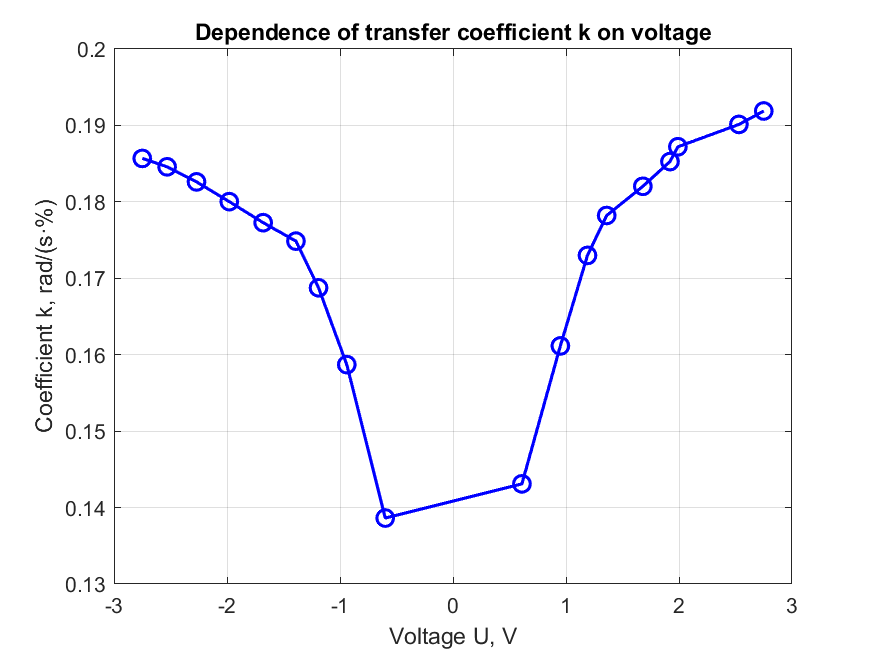
\includegraphics[width=0.9\textwidth]{../matlab/graphs/parameters/k.png}
    \caption{Зависимость коэффициента передачи $k$ от напряжения.}
    \label{fig:k}
\end{figure}

На рис.~\ref{fig:Tm} показана зависимость постоянной времени $T_m$ от напряжения. Постоянная времени остаётся приблизительно постоянной, что соответствует теории.

\begin{figure}[H]
    \centering
    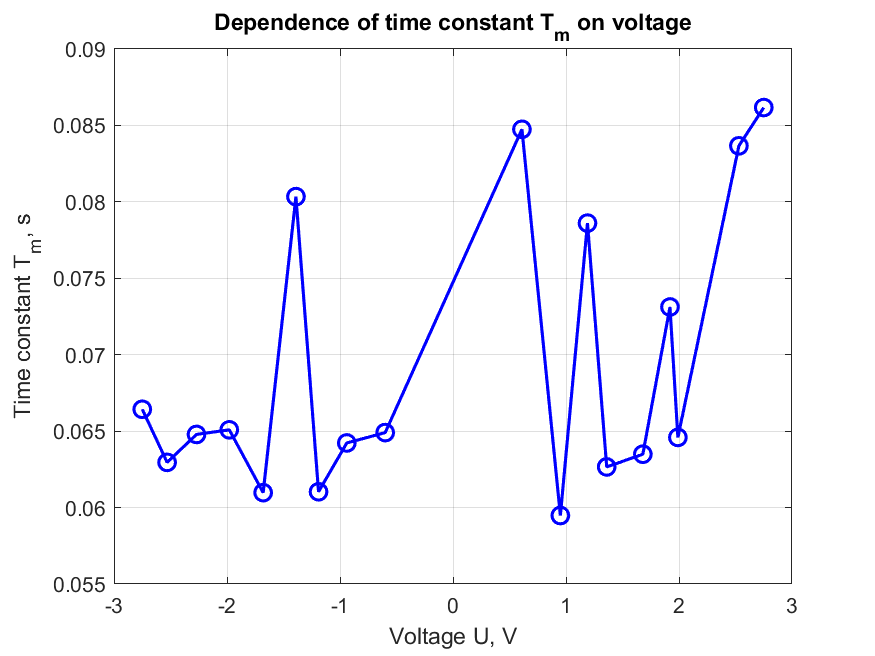
\includegraphics[width=0.9\textwidth]{../matlab/graphs/parameters/Tm.png}
    \caption{Зависимость постоянной времени $T_m$ от напряжения.}
    \label{fig:Tm}
\end{figure}

На рис.~\ref{fig:omega} показана установившаяся угловая скорость в зависимости от напряжения. Зависимость близка к линейной.

\begin{figure}[H]
    \centering
    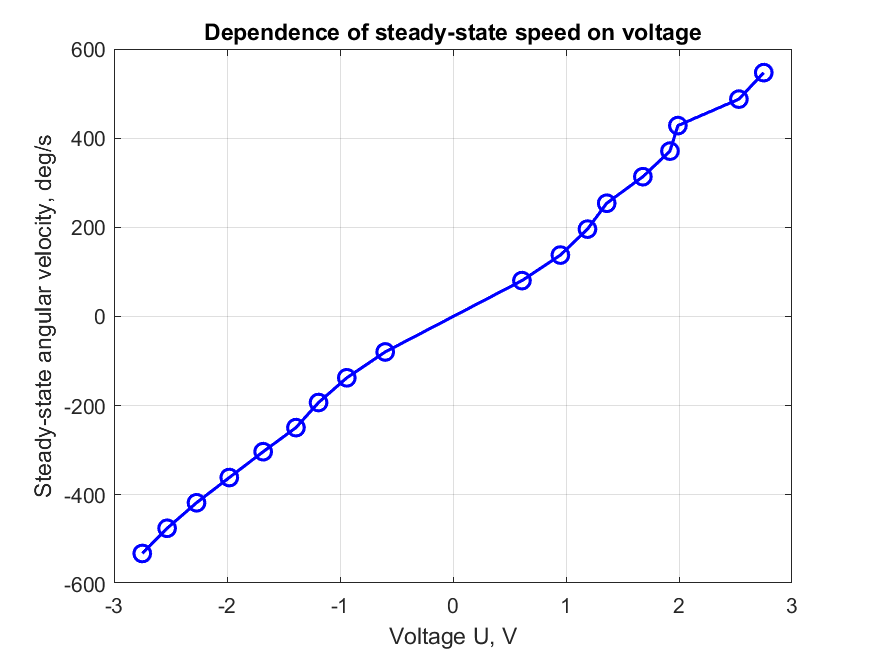
\includegraphics[width=0.9\textwidth]{../matlab/graphs/parameters/omega_steady.png}
    \caption{Установившаяся угловая скорость в зависимости от напряжения.}
    \label{fig:omega}
\end{figure}

\section{Расчёт конструктивных постоянных}


\subsection{Определение конструктивной постоянной $k_e$ из статической характеристики}

Согласно заданию (п. 2.6), коэффициент $k_e$ определяется из статической характеристики
двигателя — зависимости установившейся угловой скорости $\omega_{\text{уст}}$ от приложенного напряжения $U$.
Для каждого уровня управляющего сигнала были определены установившиеся значения
угловой скорости (табл.~\ref{tab:omega_steady}).

\begin{table}[H]
    \centering
    \caption{Установившаяся угловая скорость при различных напряжениях}
    \label{tab:omega_steady}
    \begin{tabular}{|c|c|c|}
        \hline
        \textbf{Напряжение $U$, В} & \textbf{$\omega_{\text{уст}}$, град/с} & \textbf{$\omega_{\text{уст}}$, рад/с} \\
        \hline
        2,75 & 495,2 & 8,64 \\
        2,53 & 451,8 & 7,88 \\
        2,27 & 405,3 & 7,07 \\
        1,98 & 353,6 & 6,17 \\
        1,68 & 300,1 & 5,24 \\
        1,39 & 248,5 & 4,34 \\
        1,19 & 212,8 & 3,71 \\
        0,95 & 169,9 & 2,96 \\
        0,61 & 109,2 & 1,91 \\
        \hline
    \end{tabular}
\end{table}

На рис.~\ref{fig:ke_static} представлена зависимость $U(\omega_{\text{уст}})$. Аппроксимация
экспериментальных точек прямой, проходящей через начало координат, выполнена методом
наименьших квадратов:

\begin{equation}
    k_e = \frac{\sum U_i \omega_i}{\sum \omega_i^2} \approx 0,303\ \text{В·с/рад}.
\end{equation}

\begin{figure}[H]
    \centering
    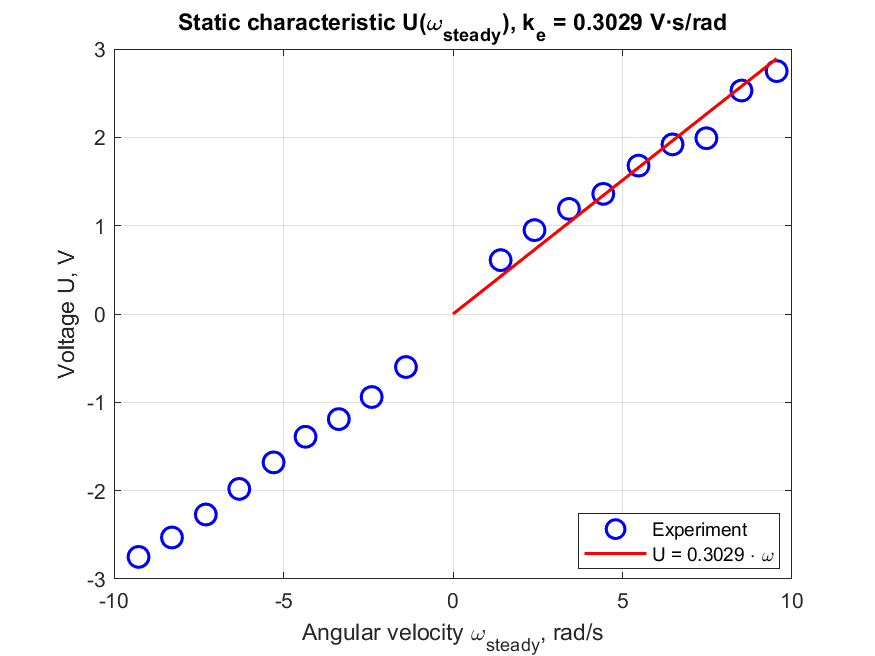
\includegraphics[width=0.8\textwidth]{../matlab/graphs/static/U_vs_omega_steady.png}
    \caption{Зависимость напряжения от установившейся угловой скорости}
    \label{fig:ke_static}
\end{figure}

Для двигателя постоянного тока с постоянными магнитами выполняется равенство
$k_m = k_e$, следовательно $k_m = 0,303$ Н·м/А.

\subsection{Альтернативные способы оценки $k_e$}

Для проверки полученного значения $k_e$ были использованы два альтернативных подхода.

\textbf{Способ 1 (через статический коэффициент передачи $k$):}
\begin{equation}
    k_e = \frac{U_{\text{max}}}{100 \cdot k} = \frac{9}{100 \cdot 0,1746} \approx 0,515\ \text{В·с/рад}.
\end{equation}

\textbf{Способ 2 (через постоянную времени $T_m$):}
\begin{equation}
    k_e = \sqrt{\frac{JR}{T_m}} = \sqrt{\frac{2,39 \times 10^{-3} \cdot 4,42}{0,0693}} \approx 0,390\ \text{В·с/рад}.
\end{equation}

\subsection{Анализ расхождений}

Расхождение между значениями $k_e$, полученными разными способами, объясняется следующими причинами:

\begin{itemize}
    \item Значение $k_e = 0,303$ В·с/рад получено \textbf{непосредственно из статической характеристики} $U(\omega_{\text{уст}})$ и является наиболее надёжным, так как не зависит от аппроксимации динамических процессов.

    \item Значение $k_e = 0,515$ В·с/рад получено косвенно через статический коэффициент передачи $k$. Погрешность связана с тем, что при малых управляющих сигналах ($\pm10\%\ldots\pm20\%$) наблюдается нелинейность ШИМ-регулирования, что влияет на усреднённое значение $k$.

    \item Значение $k_e = 0,390$ В·с/рад получено косвенно через постоянную времени $T_m$. Этот способ наиболее чувствителен к погрешностям аппроксимации переходного процесса угла, а также к неучтённому трению в редукторе, которое занижает оценку $T_m$.
\end{itemize}

\textbf{Итоговое значение:} в качестве конструктивной постоянной двигателя принимаем
значение, полученное из статической характеристики:
\begin{equation}
    \boxed{k_e = k_m = 0,303\ \text{В·с/рад}}.
\end{equation}

\section{Верификация параметров в Simulink}

Для проверки полученных параметров была построена Simulink-модель (рис.~\ref{fig:simulink_scheme}), соответствующая полной модели «вход-состояние».

\begin{figure}[H]
    \centering
    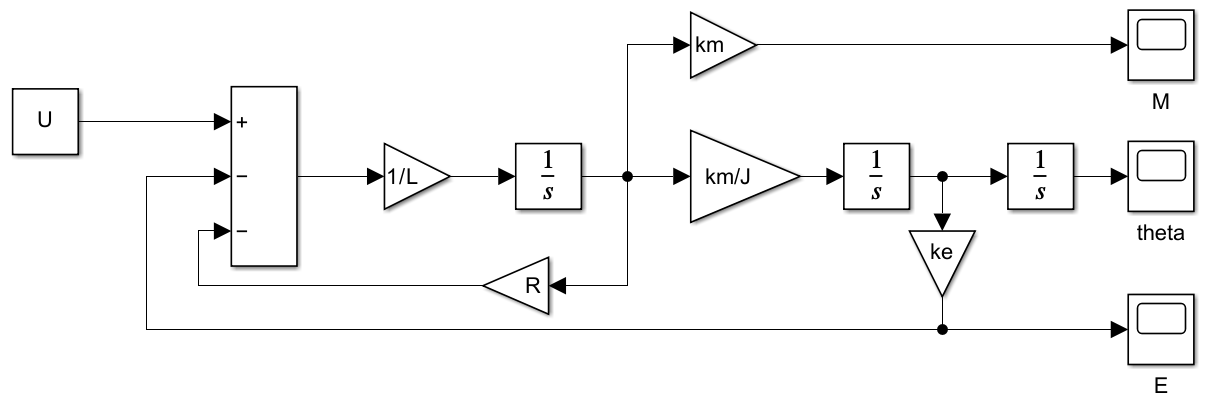
\includegraphics[width=0.8\textwidth]{shema_2.png}
    \caption{Схема моделирования процесса разгона ненагруженного двигателя в Simulink.}
    \label{fig:simulink_scheme}
\end{figure}

На рис.~\ref{fig:comparison} приведено сравнение экспериментальных данных с результатами моделирования для угловой скорости и угла поворота.

\begin{figure}[H]
    \centering
    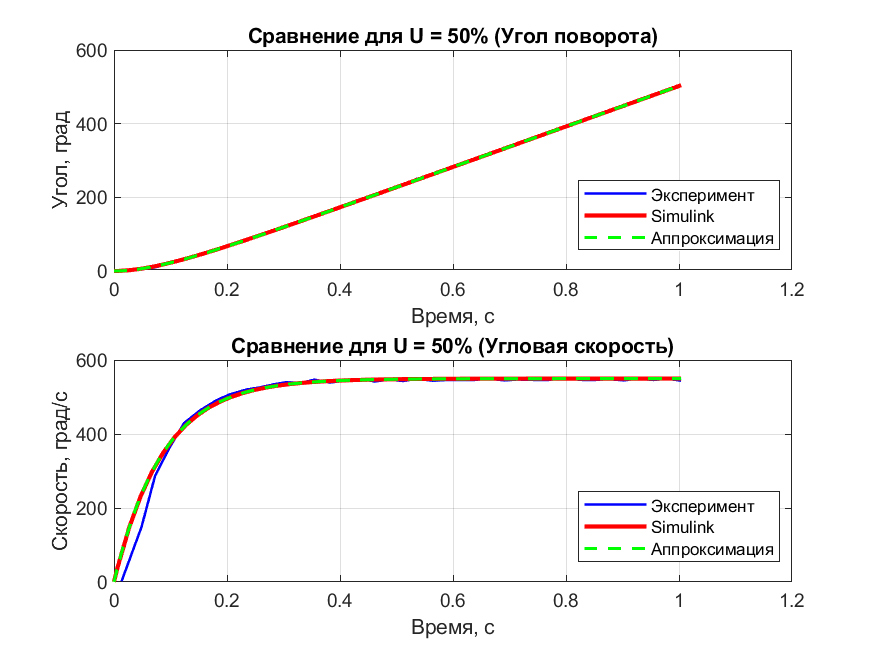
\includegraphics[width=0.9\textwidth]{../matlab/graphs/comparison/comparison_50.png}
    \caption{Сравнение экспериментальных данных, аппроксимации и Simulink-модели для $U = +50\%$.}
    \label{fig:comparison}
\end{figure}

На рис.~\ref{fig:sim_current} показан моделируемый переходный процесс тока в обмотке якоря.

\begin{figure}[H]
    \centering
    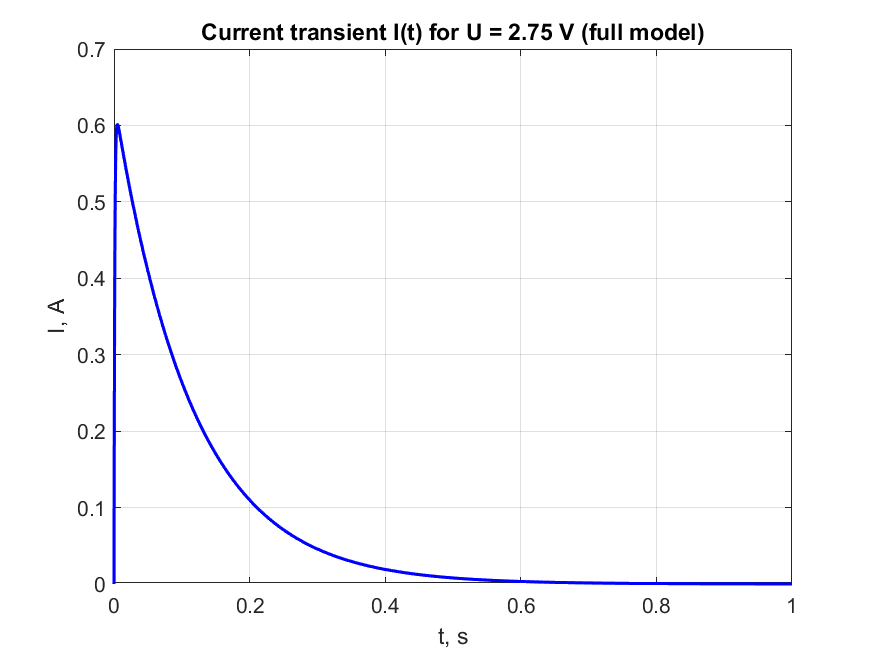
\includegraphics[width=0.8\textwidth]{../matlab/graphs/ode_current.png}
    \caption{Переходный процесс тока в обмотке якоря по полной модели.}
    \label{fig:sim_current}
\end{figure}

\section{Сравнение с лабораторной работой №1}

В лабораторной работе №1 определялись параметры двигателя при управляющем сигнале в диапазоне $\pm 20\% \dots \pm 100\%$. В работе №2 диапазон расширен до $\pm 10\% \dots \pm 50\%$ для исследования нелинейностей в области малых сигналов.

Сравнение средних значений представлено в табл.~\ref{tab:comparison}.

\begin{table}[H]
    \centering
    \caption{Сравнение параметров, полученных в lab\_1 и lab\_2}
    \label{tab:comparison}
    \begin{tabular}{|l|c|c|}
        \hline
        \textbf{Параметр} & \textbf{lab\_1} & \textbf{lab\_2} \\
        \hline
        $k$ (рад/(с·\%))  & 0,1802 & 0,1741 \\
        $T_m$ (с)         & 0,0806 & 0,0768 \\
        $R$ (Ом)          & $-$    & 4,39 \\
        $k_e$ (В·с/рад)   & $-$    & 0,303 \\

        \hline
    \end{tabular}
\end{table}

Значения $k$ и $T_m$ хорошо согласуются между работами, что подтверждает воспроизводимость экспериментальной методики. Небольшое расхождение объясняется:
\begin{itemize}
    \item различным диапазоном управляющих сигналов;
    \item влиянием трения в редукторе, более заметным при малых сигналах;
    \item дискретностью ШИМ-регулирования.
\end{itemize}

\section{Выводы}

В ходе выполнения лабораторной работы все поставленные задачи были решены:

\begin{enumerate}
    \item Изучена полная математическая модель двигателя постоянного тока с учётом индуктивности обмоток ($L = 0.0047$ Гн).
    \item Снята вольтамперная характеристика для 18 уровней управляющего сигнала в диапазоне от $-50\%$ до $+50\%$.
    \item Определено активное сопротивление обмоток $R = 4.39$ Ом.
    \item По переходным характеристикам идентифицированы параметры модели: средний статический коэффициент передачи $k = 0.1741$ рад/(с·\%), средняя постоянная времени $T_m = 0.0768$ с.
    \item На основе геометрических параметров ротора и передаточного отношения редуктора рассчитан момент инерции $J = 2.39 \times 10^{-3}$ кг·м$^2$.
\item Вычислены конструктивные постоянные двигателя: $k_e = k_m = 0,303$ В·с/рад (основной результат, полученный из статической характеристики $U(\omega_{\text{уст}})$).
    \item Построена Simulink-модель, подтвердившая адекватность полученных параметров.
    \item Результаты согласуются с данными лабораторной работы №1, что подтверждает надёжность методики.
\end{enumerate}

Таким образом, цель работы достигнута: на основе экспериментальных данных определены ключевые параметры полной математической модели двигателя EV3, необходимые для дальнейшего управления и моделирования системы.

\newpage

\section*{Приложение А: Программный код}

\subsection*{Python-скрипт для сбора данных}

\begin{lstlisting}[language=Python, caption=Скрипт для сбора экспериментальных данных]
from ev3dev2.motor import LargeMotor, OUTPUT_B
import time

motorA = LargeMotor(OUTPUT_B)
voltages = [50, 45, 40, 35, 30, 25, 20, 15, 10,
           -10, -15, -20, -25, -30, -35, -40, -45, -50]

try:
    for vol in voltages:
        timeStart = time.time()
        startPos = motorA.position
        name = "data" + str(vol) + ".txt"
        file = open(name, "w")

        while True:
            timeNow = time.time() - timeStart
            motorA.run_direct(duty_cycle_sp=vol)
            pos = motorA.position - startPos
            file.write(str(timeNow) + " " + str(pos)
                       + " " + str(motorA.speed) + "\n")

            if timeNow > 1:
                motorA.run_direct(duty_cycle_sp=0)
                break

            time.sleep(0.01)

        file.close()
        motorA.stop(stop_action='brake')
        time.sleep(1.5)

except Exception as e:
    raise e

finally:
    motorA.stop(stop_action='brake')
\end{lstlisting}

\subsection*{MATLAB-скрипт обработки данных}

\begin{lstlisting}[language=MatLab, caption=Основной скрипт обработки данных и идентификации параметров]
clear; clc; close all;

%% ========================
% 1. ПАРАМЕТРЫ И ДАННЫЕ U-I
% ========================
csv_file = '../U_I.csv';

m = 15.7e-3;        % kg
r = 11.5e-3;        % m
gear_ratio = 48;
L = 0.0047;         % H
Umax = 9.0;         % V

T = readtable(csv_file, 'Delimiter', ';');
U = str2double(strrep(string(T{:,2}), ',', '.'));
I = str2double(strrep(string(T{:,3}), ',', '.'));

R = sum(U .* I) / sum(I.^2);

J_ed = (m * r^2) / 2;
J = gear_ratio^2 * J_ed;

assignin('base', 'J', J);
assignin('base', 'L', L);
assignin('base', 'R', R);

fprintf('===== ПАРАМЕТРЫ =====\n');
fprintf('R = %.4f Ohm\n', R);
fprintf('J = %.6f kg*m^2\n', J);

%% ========================
% 2. ОБРАБОТКА ДАННЫХ
% ========================
data_folder = '../data';
graphs_folder = 'graphs';
if ~exist(graphs_folder, 'dir'), mkdir(graphs_folder); end

angles_folder = fullfile(graphs_folder, 'angles');
velocities_folder = fullfile(graphs_folder, 'velocities');
comparison_folder = fullfile(graphs_folder, 'comparison');
parameters_folder = fullfile(graphs_folder, 'parameters');

for d = {angles_folder, velocities_folder, comparison_folder, parameters_folder}
    if ~exist(d{1}, 'dir'), mkdir(d{1}); end
end

voltages = [-50, -45, -40, -35, -30, -25, -20, -15, -10, ...
            10, 15, 20, 25, 30, 35, 40, 45, 50];
n_files = length(voltages);

k_all = NaN(n_files, 1);
Tm_all = NaN(n_files, 1);
ke_all = NaN(n_files, 1);
km_all = NaN(n_files, 1);

%% ========================
% 3. ГРАФИКИ: ВСЕ УГЛЫ И ВСЕ СКОРОСТИ НА ОДНОМ
% ========================
figure(1); clf; hold on;
colors = jet(n_files);
figure(2); clf; hold on;

leg_angle = cell(n_files, 1);
leg_vel = cell(n_files, 1);

for i = 1:n_files
    U_pr = voltages(i);
    filename = fullfile(data_folder, sprintf('data%d.txt', U_pr));
    if ~isfile(filename)
        filename = fullfile(data_folder, sprintf('data%d', U_pr));
        if ~isfile(filename), continue; end
    end

    data = readmatrix(filename);
    if isempty(data), continue; end

    time = data(:, 1);
    angle_deg = data(:, 2);
    omega_deg = data(:, 3);
    angle_rad = angle_deg * pi / 180;

    figure(1);
    plot(time, angle_deg, 'Color', colors(i,:), 'LineWidth', 1.2);
    leg_angle{i} = sprintf('U = %d%%', U_pr);

    figure(2);
    plot(time, omega_deg, 'Color', colors(i,:), 'LineWidth', 1.2);
    leg_vel{i} = sprintf('U = %d%%', U_pr);

    fun = @(par, t) U_pr * par(1) * (t - par(2) * (1 - exp(-t/par(2))));
    opts = optimoptions('lsqcurvefit', 'Display', 'off');

    try
        p = lsqcurvefit(fun, [15, 0.06], time, angle_rad, [], [], opts);
        k = p(1);
        Tm = p(2);
        k_all(i) = k;
        Tm_all(i) = Tm;

        ke_curr = Umax / (100 * k);
        km_curr = J * R / (Tm * ke_curr);
        ke_all(i) = ke_curr;
        km_all(i) = km_curr;

        t_apr = linspace(0, max(time), 200);
        theta_apr = fun([k, Tm], t_apr) * 180 / pi;
        omega_apr = k * U_pr * (1 - exp(-t_apr/Tm)) * 180 / pi;

        figure(1);
        plot(t_apr, theta_apr, '--', 'Color', colors(i,:), 'LineWidth', 0.8);

        figure(2);
        plot(t_apr, omega_apr, '--', 'Color', colors(i,:), 'LineWidth', 0.8);
    catch
    end
end

figure(1);
xlabel('Time, s'); ylabel('Angle, deg');
title('Transition processes of rotation angle');
grid on;
legend(leg_angle, 'Location', 'eastoutside', 'FontSize', 7);
saveas(gcf, fullfile(graphs_folder, 'all_angles.png'));

figure(2);
xlabel('Time, s'); ylabel('Angular velocity, deg/s');
title('Transition processes of angular velocity');
grid on;
legend(leg_vel, 'Location', 'eastoutside', 'FontSize', 7);
saveas(gcf, fullfile(graphs_folder, 'all_velocities.png'));

%% ========================
% 4. ИНДИВИДУАЛЬНЫЕ ГРАФИКИ
% ========================
for i = 1:n_files
    if isnan(k_all(i)), continue; end

    U_pr = voltages(i);
    filename = fullfile(data_folder, sprintf('data%d.txt', U_pr));
    if ~isfile(filename), filename = fullfile(data_folder, sprintf('data%d', U_pr)); end

    data = readmatrix(filename);
    time = data(:, 1);

    figure(10 + i);
    plot(time, data(:,2), 'b.-', 'LineWidth', 1.2, 'MarkerSize', 8); hold on;
    t_apr = 0:0.01:max(time);
    theta_apr = U_pr * k_all(i) * (t_apr - Tm_all(i) * (1 - exp(-t_apr/Tm_all(i)))) * 180 / pi;
    plot(t_apr, theta_apr, 'r-', 'LineWidth', 1);
    title(sprintf('Angle U = %d%%, k = %.3f, Tm = %.3f s', U_pr, k_all(i), Tm_all(i)));
    legend('Experiment', 'Approx'); grid on;
    saveas(gcf, fullfile(angles_folder, sprintf('angle_%d.png', U_pr)));

    figure(30 + i);
    plot(time, data(:,3), 'b.-', 'LineWidth', 1.2, 'MarkerSize', 8); hold on;
    omega_apr = k_all(i) * U_pr * (1 - exp(-t_apr/Tm_all(i))) * 180 / pi;
    plot(t_apr, omega_apr, 'r-', 'LineWidth', 1);
    title(sprintf('Speed U = %d%%, k = %.3f, Tm = %.3f s', U_pr, k_all(i), Tm_all(i)));
    legend('Experiment', 'Approx'); grid on;
    saveas(gcf, fullfile(velocities_folder, sprintf('velocity_%d.png', U_pr)));
end

%% ========================
% 5. ВОЛЬТ-АМПЕРНАЯ ХАРАКТЕРИСТИКА
% ========================
I_line = linspace(min(I), max(I), 200);
U_line = R * I_line;

figure('Name','U(I)');
plot(I, U, 'b.-', 'LineWidth', 1.5, 'MarkerSize', 12); hold on;
plot(I_line, U_line, 'r-', 'LineWidth', 1);
grid on;
xlabel('Current I, A'); ylabel('Voltage U, V');
title('Volt-ampere characteristic');
legend('Experimental', sprintf('U = %.4f I', R), 'Location', 'best');
saveas(gcf, fullfile(graphs_folder, 'U_I_dependence.png'));

%% ========================
% 6. ПЕРЕХОДНЫЙ ПРОЦЕСС ТОКА (ODE45)
% ========================
valid = ~isnan(ke_all);
ke_mean = mean(ke_all(valid));
km_mean = ke_mean;

assignin('base', 'ke', ke_mean);
assignin('base', 'km', km_mean);

Uctrl = 2.75;
tspan = [0 1];

f = @(t,x) [ (km_mean/J) * x(2);
             (1/L)*Uctrl - (ke_mean/L)*x(1) - (R/L)*x(2);
             x(1) ];

[t, x] = ode45(f, tspan, [0; 0; 0]);

figure('Name','Current');
plot(t, x(:,2), 'LineWidth', 1.5);
grid on; xlabel('t, s'); ylabel('I, A');
title('Current transient I(t)');
saveas(gcf, fullfile(graphs_folder, 'ode_current.png'));

%% ========================
% 7. SIMULINK ВЕРИФИКАЦИЯ
% ========================
if license('test', 'Simulink')
    modelName = 'temp_motor_model';
    if bdIsLoaded(modelName), close_system(modelName, 0); end
    if isfile([modelName '.slx']), delete([modelName '.slx']); end

    create_motor_sim_model(modelName);

    for i = 1:n_files
        if isnan(k_all(i)), continue; end

        U_pr = voltages(i);
        assignin('base', 'k_sim', k_all(i));
        assignin('base', 'Tm_sim', Tm_all(i));
        assignin('base', 'U_sim', U_pr);

        filename = fullfile(data_folder, sprintf('data%d.txt', U_pr));
        if ~isfile(filename), filename = fullfile(data_folder, sprintf('data%d', U_pr)); end
        data = readmatrix(filename);
        time_exp = data(:, 1);
        t_end = max(time_exp);

        set_param(modelName, 'StopTime', num2str(t_end));

        try
            sim(modelName);
            pause(0.3);

            if isfile('omega_data.mat') && isfile('theta_data.mat')
                omega_mat = load('omega_data.mat');
                theta_mat = load('theta_data.mat');
                omega_fields = fieldnames(omega_mat);
                theta_fields = fieldnames(theta_mat);
                omega_var = omega_mat.(omega_fields{1});
                theta_var = theta_mat.(theta_fields{1});
                time_sim = omega_var.Time(:);
                omega_sim = omega_var.Data(:);
                theta_sim = theta_var.Data(:);

                figure(200 + i);

                subplot(2,1,1);
                plot(time_exp, data(:,2), 'b-', 'LineWidth', 1.2); hold on;
                plot(time_sim, theta_sim * 180/pi, 'r-', 'LineWidth', 2);
                t_apr = linspace(0, t_end, 200);
                theta_apr = U_pr * k_all(i) * (t_apr - Tm_all(i) * (1 - exp(-t_apr/Tm_all(i)))) * 180 / pi;
                plot(t_apr, theta_apr, 'g--', 'LineWidth', 1.5);
                xlabel('Time, s'); ylabel('Angle, deg');
                title(sprintf('Angle comparison U = %d%%', U_pr));
                legend('Experiment', 'Simulink', 'Approximation'); grid on;

                subplot(2,1,2);
                plot(time_exp, data(:,3), 'b-', 'LineWidth', 1.2); hold on;
                plot(time_sim, omega_sim * 180/pi, 'r-', 'LineWidth', 2);
                omega_apr = k_all(i) * U_pr * (1 - exp(-t_apr/Tm_all(i))) * 180 / pi;
                plot(t_apr, omega_apr, 'g--', 'LineWidth', 1.5);
                xlabel('Time, s'); ylabel('Speed, deg/s');
                title(sprintf('Speed comparison U = %d%%', U_pr));
                legend('Experiment', 'Simulink', 'Approximation'); grid on;

                saveas(gcf, fullfile(comparison_folder, sprintf('comparison_%d.png', U_pr)));
                close(gcf);
            end

            if isfile('omega_data.mat'), delete('omega_data.mat'); end
            if isfile('theta_data.mat'), delete('theta_data.mat'); end
        catch
        end
    end

    if bdIsLoaded(modelName), close_system(modelName, 0); end
else
    fprintf('Simulink not available, skipping verification.\n');
end

%% ========================
% 8. ВЫВОД СРЕДНИХ ЗНАЧЕНИЙ
% ========================
valid = ~isnan(k_all) & ~isnan(Tm_all);
k_mean = mean(k_all(valid));
Tm_mean = mean(Tm_all(valid));
ke_mean = mean(ke_all(valid));
km_mean = ke_mean;

fprintf('\n===== СРЕДНИЕ ПАРАМЕТРЫ ДЛЯ ОТЧЁТА =====\n');
fprintf('k   = %.4f rad/(s%%)\n', k_mean);
fprintf('Tm  = %.4f s\n', Tm_mean);
fprintf('ke  = %.4f V*s/rad\n', ke_mean);
fprintf('km  = %.4f N*m/A\n', km_mean);
fprintf('R   = %.4f Ohm\n', R);
fprintf('J   = %.6f kg*m^2\n', J);
fprintf('L   = %.4f H\n', L);

disp('Обработка завершена.');

%% ========================
% 9. ФУНКЦИЯ СОЗДАНИЯ SIMULINK МОДЕЛИ
% ========================
function create_motor_sim_model(modelName)
    new_system(modelName);
    open_system(modelName);
    set_param(modelName, 'StopTime', '1.0', 'Solver', 'ode45');

    add_block('simulink/Sources/Constant', [modelName '/U']);
    set_param([modelName '/U'], 'Value', 'U_sim');

    add_block('simulink/Math Operations/Gain', [modelName '/Gain_k']);
    set_param([modelName '/Gain_k'], 'Gain', 'k_sim');

    add_block('simulink/Math Operations/Sum', [modelName '/Sum']);
    set_param([modelName '/Sum'], 'Inputs', '+-');

    add_block('simulink/Math Operations/Gain', [modelName '/Gain_1Tm']);
    set_param([modelName '/Gain_1Tm'], 'Gain', '1/Tm_sim');

    add_block('simulink/Continuous/Integrator', [modelName '/Integ_omega']);
    set_param([modelName '/Integ_omega'], 'InitialCondition', '0');

    add_block('simulink/Continuous/Integrator', [modelName '/Integ_theta']);
    set_param([modelName '/Integ_theta'], 'InitialCondition', '0');

    add_block('simulink/Sinks/To File', [modelName '/ToFile_omega']);
    set_param([modelName '/ToFile_omega'], 'Filename', 'omega_data.mat');

    add_block('simulink/Sinks/To File', [modelName '/ToFile_theta']);
    set_param([modelName '/ToFile_theta'], 'Filename', 'theta_data.mat');

    add_line(modelName, 'U/1', 'Gain_k/1');
    add_line(modelName, 'Gain_k/1', 'Sum/1');
    add_line(modelName, 'Integ_omega/1', 'Sum/2');
    add_line(modelName, 'Sum/1', 'Gain_1Tm/1');
    add_line(modelName, 'Gain_1Tm/1', 'Integ_omega/1');
    add_line(modelName, 'Integ_omega/1', 'Integ_theta/1');
    add_line(modelName, 'Integ_omega/1', 'ToFile_omega/1');
    add_line(modelName, 'Integ_theta/1', 'ToFile_theta/1');

    save_system(modelName);
end
\end{lstlisting}

\end{document}